\documentclass[11pt]{article}

\usepackage[margin=1in]{geometry}
\usepackage{amsmath}
\usepackage{amssymb}
\usepackage{graphicx}
\usepackage{hyperref}
\usepackage{booktabs}
\usepackage{caption}
\usepackage{wrapfig}

\title{VDF Classification: Investigation Progress}
\author{}
\date{\today}

\begin{document}
\maketitle

\begin{abstract}
This study reports preliminary results on clusterization of the
Vlasiator 2D global simulation, with the idea of identification of the
magnetospheric regions. The practical goal for now is to sanity-check
the extraction, labelling, and PCA pipelines end to end before scaling
to a full production run. Section~\ref{sec:data-processing} describes
the expert-based region detection and the labelling strategies (116
VDFs across six substances). Section~\ref{sec:pca} reports blind
PCA+KMeans clustering on the Hermite spectra of the VDFs, with
lower-order physical moments (density, bulk velocity, anisotropic
thermal velocity) added as explicit features. The best-scoring split
($k=2$) recovers a cluster containing \emph{all} \texttt{magnetosheath}
and \emph{all} \texttt{current\_layer} samples (100\% recall of both),
at 81\% purity within that cluster -- these VDFs could be considered
``disturbed'' plasma. The complementary cluster is 100\% pure
calm-plasma labels.
\end{abstract}

\tableofcontents

% ---------------------------------------------------------------------
\section{Data processing}
\label{sec:data-processing}
% Stage: selecting where VDFs are pulled from a snapshot, and assigning
% each one its physics-derived ground-truth label. Corresponds to
% TESTING.md Stages 1-3 ("data extraction" / "processing" / "labelling").

\subsection{Smoke-test snapshot and VDF extraction}
All results below are from \texttt{RUN\_ID = smoke\_test}: one local
Vlasiator timestep (\texttt{bulk.0003408.vlsv}), a sparse, coarse 2D
$xz$-plane run ($y \equiv 0$) chosen deliberately for fast pipeline
iteration rather than physical realism -- $\sim$2880 VDF-carrying cells
over the whole domain, $\sim$2.35~$R_E$ spacing. Extraction was
restricted to a search box \texttt{SPATIAL\_BOXRE~=~[-30, 30, -5, 5]}
$R_E$ ($x$, $z$), a band straddling the dayside magnetopause and the
near tail. 116 VDF-carrying cells fell inside that box and were
extracted with \texttt{VdfExtractor} at the snapshot's native
velocity-mesh resolution ($4\times4\times4$ blocks/cell). Figure
\ref{fig:all-vdfs} shows their spatial distribution together with the
labels assigned in Section~\ref{sec:labelling}.

\begin{figure}[h]
\centering
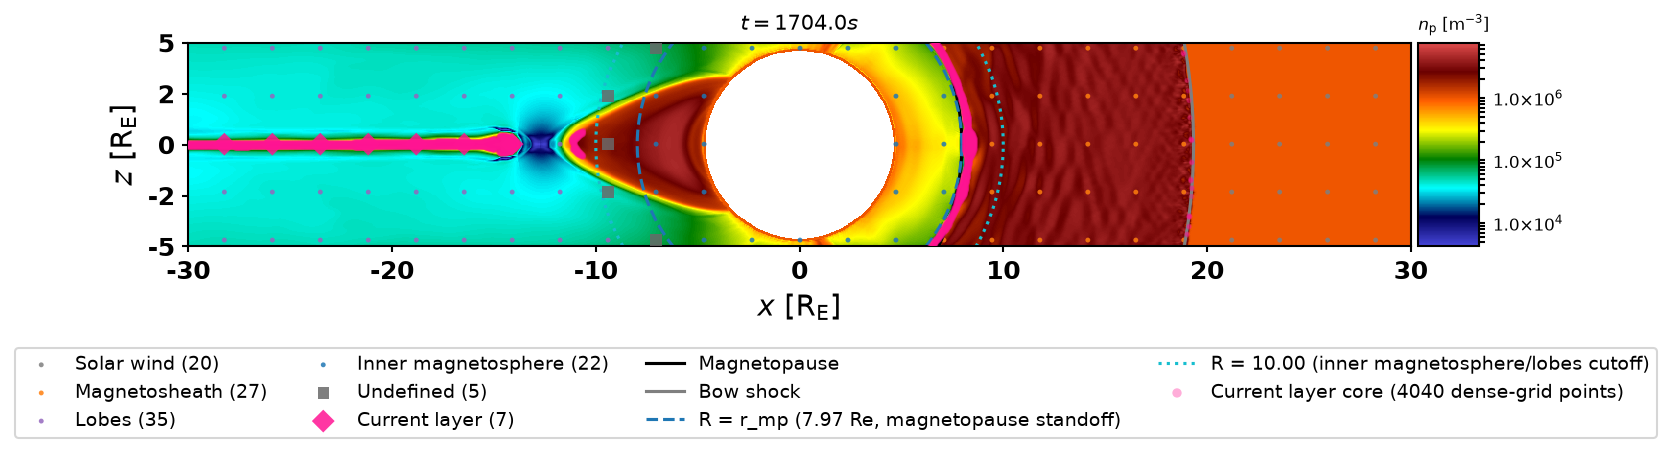
\includegraphics[width=0.85\textwidth]{./images/all_vdfs.png}
\caption{Extracted VDF cells, colored by ground-truth label, smoke\_test
run. Blue dashed circle: fitted Shue standoff $r_{mp}$. Cyan dotted circle:
\texttt{lobe\_r\_min\_re}. Pink dot cloud: the current-layer core's
dense-grid extent; pink diamonds: the VDF cells actually labelled
\texttt{current\_layer}.}
\label{fig:all-vdfs}
\end{figure}

\subsection{Labelling}
\label{sec:labelling}

\subsubsection{Finding the magnetopause and bow shock}
Both boundaries are located by a 1D density scan along the Sun-Earth
line ($+x$, $y=z=0$), from $x = 30~R_E$ (undisturbed solar wind) inward
to $x = 5~R_E$ (near Earth), sampled at 300 points
(\texttt{find\_subsolar\_point}). Moving inward, the density profile
crosses two boundaries in sequence: first a steep \emph{rise} (shocked,
compressed solar wind -- the bow shock), then, further in, a steep
\emph{drop} (from the dense sheath back down into the more tenuous
magnetosphere -- the magnetopause). Both crossings are found the same
way: the magnetopause is the grid step with the steepest drop in
$\log(\rho)$ over the whole scan; the bow shock is the steepest
\emph{rise} in $\log(\rho)$, restricted to the sunward side of the
magnetopause crossing. On this run: magnetopause at $r_{mp} \approx
7.97~R_E$ (density $1.13\times10^6 \rightarrow 1.85\times10^5$~m$^{-3}$),
bow shock at $r_{bs} \approx 19.34~R_E$ (density $1.10\times10^6
\rightarrow 2.86\times10^6$~m$^{-3}$, a $\sim$3-4$\times$ compression --
the theoretical maximum for a perpendicular MHD shock).

These two subsolar crossing distances anchor a subsolar Shue et
al.\ (1998)-shaped surface, $r(\theta) = r_{mp} \left(\frac{2}{1 +
\cos\theta}\right)^{\alpha}$, with $\theta$ measured from the Sun-Earth
line -- one surface for the magnetopause (using $r_{mp}$) and one for the
bow shock (using $r_{bs}$), both sharing the canonical flaring exponent
$\alpha = 0.58$ (this run has no solar wind monitor to fit $\alpha$
from locally). This is a standard empirical parametrization of how both
boundaries flare away from Earth off the Sun-Earth line, fitted here
from a single subsolar density cut rather than a full boundary scan.

% wrapfig cannot split a figure across a page break, and this figure is
% ~2x taller than it is wide -- the section must start high on a fresh
% page or the reserved text indent and the figure end up on different
% pages (observed, not hypothetical).
\newpage
\subsubsection{What each region is}

\begin{wrapfigure}{r}{0.40\textwidth}
\vspace{-12pt}
\centering
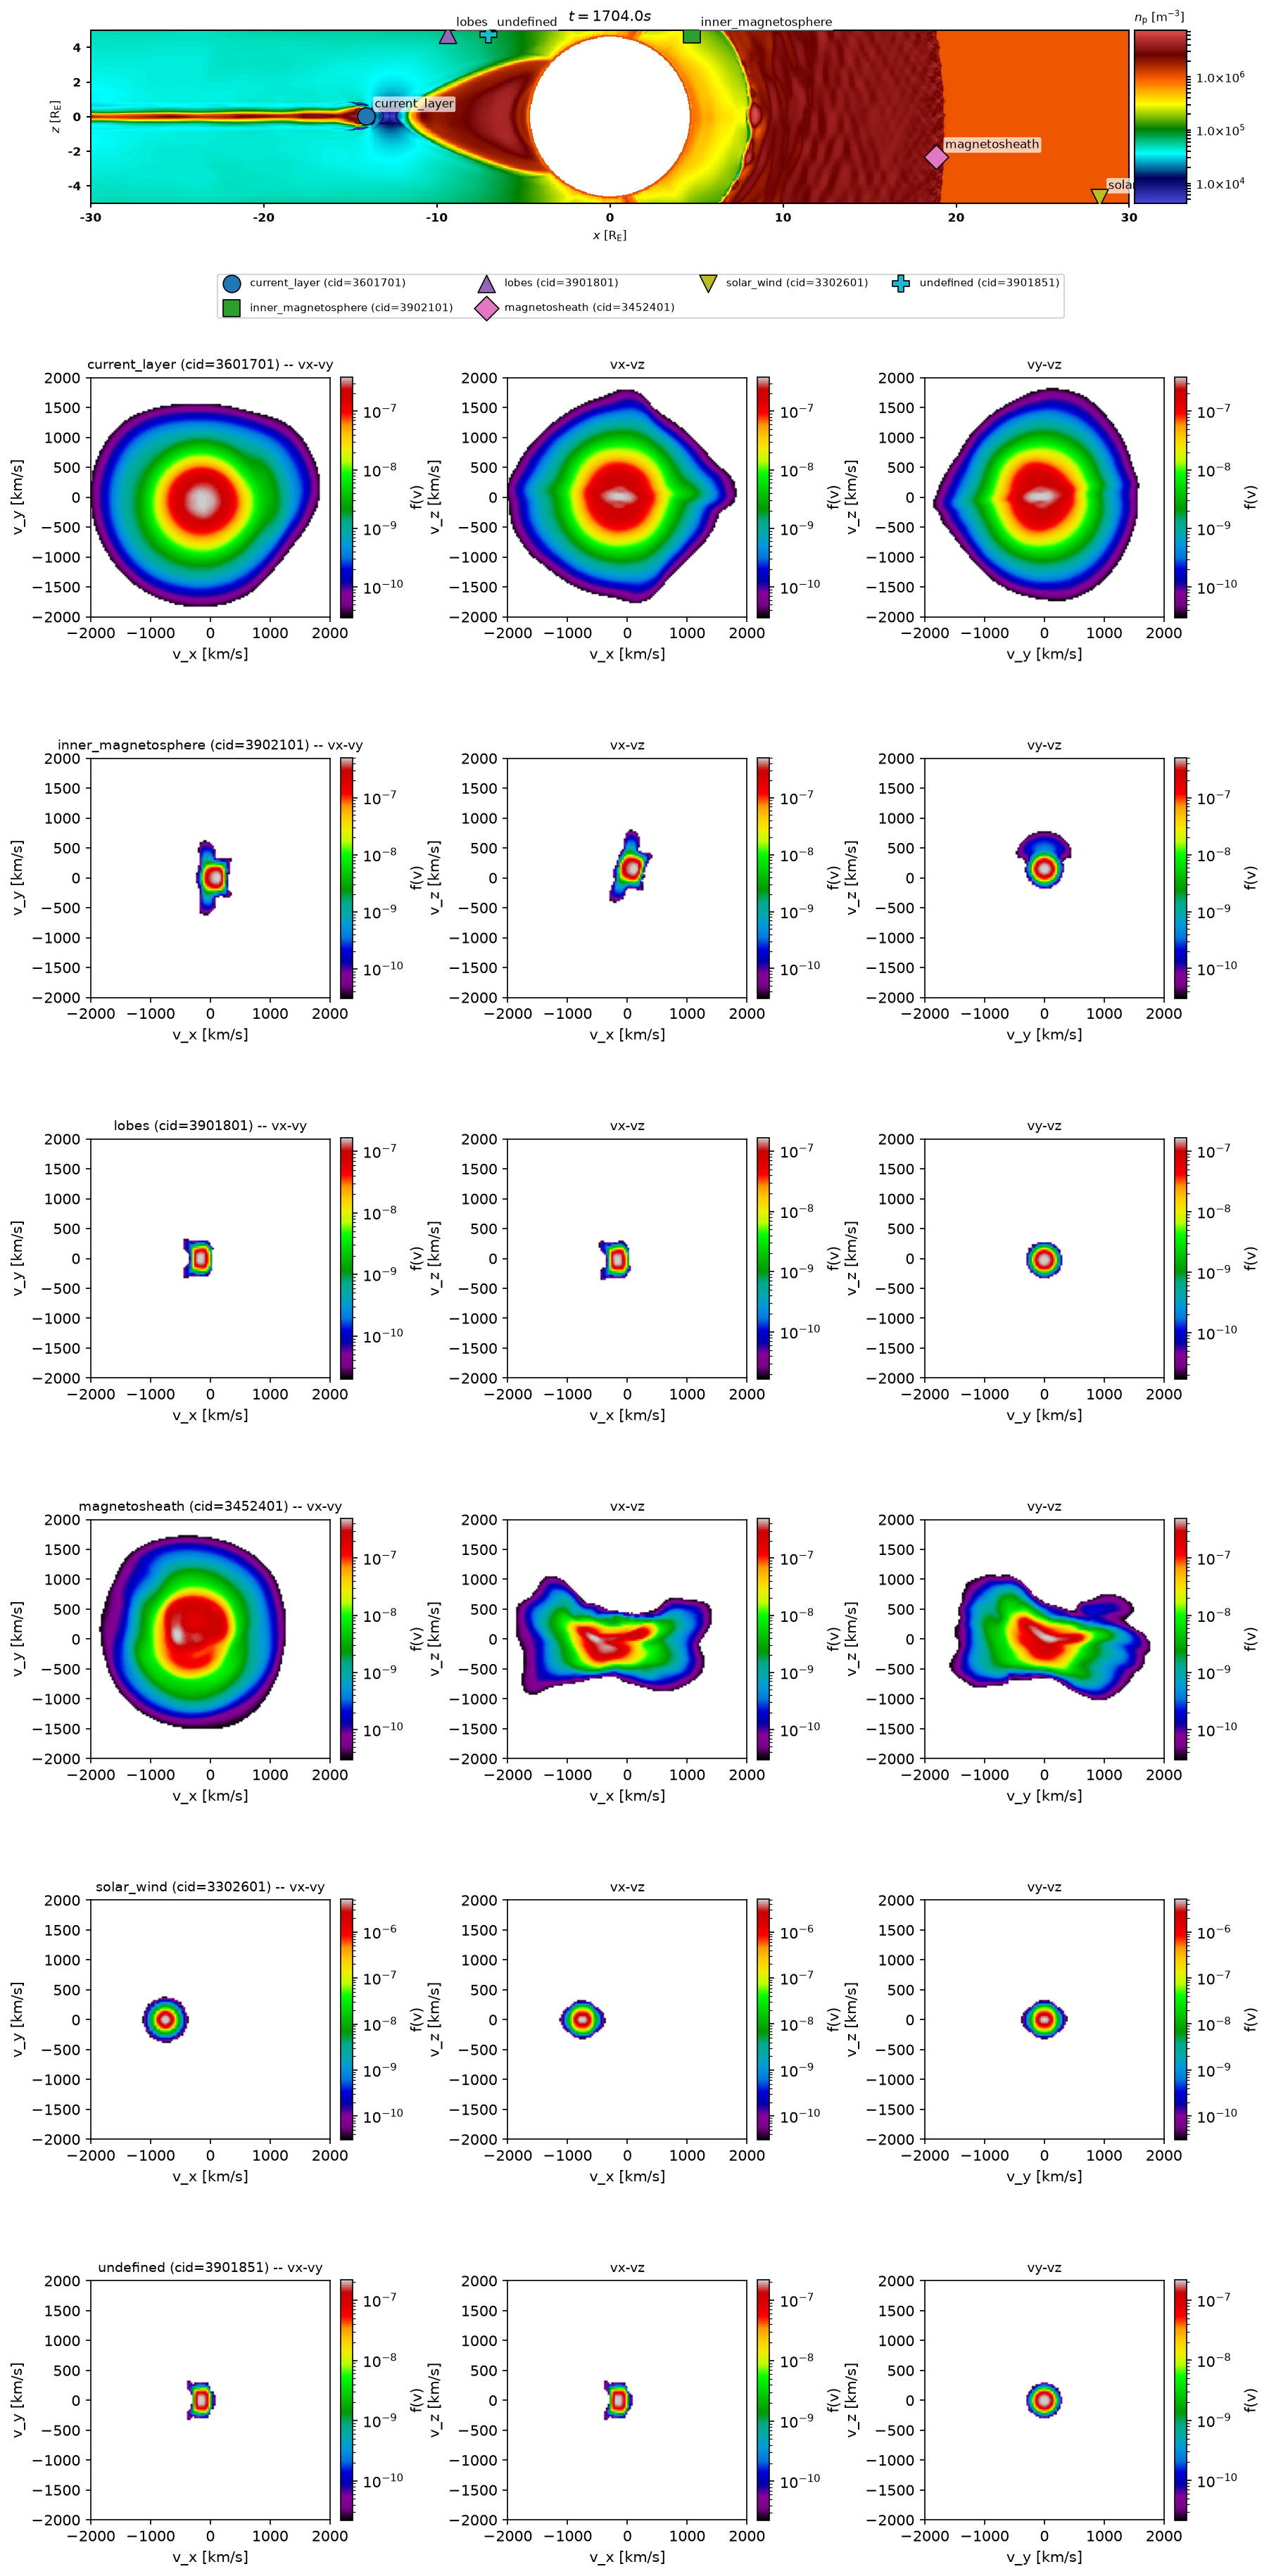
\includegraphics[width=\linewidth,trim={0.15cm 0.15cm 0.15cm 0.15cm},clip]{./images/vdf_examples.png}
\caption{Labelling verification, smoke\_test run: where each
representative VDF sits (top) and its velocity-space cuts
($v_x$-$v_y$, $v_x$-$v_z$, $v_y$-$v_z$) below.}
\label{fig:vdf-verification}
\vspace{-10pt}
\end{wrapfigure}

With both flared surfaces in hand, every extracted VDF cell is
classified by \texttt{classify\_magnetosphere\_regions} purely from its
position (and local density) relative to them:
\begin{itemize}
  \item \textbf{Solar wind}: outside the bow-shock surface -- undisturbed
  upstream plasma that hasn't yet interacted with Earth's magnetosphere.
  A fast, narrow, close-to-Maxwellian beam.
  \item \textbf{Magnetosheath}: between the bow-shock and magnetopause
  surfaces -- solar wind that has crossed the bow shock and been shocked,
  compressed, and heated. Denser and hotter than the solar wind, with a
  broader, more turbulent VDF (decelerated and deflected around the
  magnetopause).
  \item \textbf{Inner magnetosphere}: inside the magnetopause surface and
  close to Earth ($R < r_{mp}$, a simple sphere, not the flared shape) --
  dominated by Earth's dipole field, populated by trapped, quasi-thermal
  plasma.
  \item \textbf{Lobes}: inside the magnetopause surface but far from Earth
  ($R \geq$ \texttt{lobe\_r\_min\_re}, $10~R_E$ here) -- tenuous,
  open-field-line tail plasma, the coldest/most rarefied population in
  this taxonomy.
  \item \textbf{Current layer} (Section~\ref{sec:pca}'s ``disturbed''
  population, together with magnetosheath): overrides whichever of the
  other regions a cell would otherwise get, wherever a cell coincides
  with a peak-$|J|$ core cell (the only active point substance this run,
  \texttt{core\_fraction~=~0.2}, dayside/tail search boxes independent,
  cells within $6~R_E$ of Earth excluded).
  \item \textbf{Undefined}: inside the magnetopause surface, in the
  geometric gap $r_{mp} \leq R < $ \texttt{lobe\_r\_min\_re} -- $r_{mp}$ is a
  \emph{dayside-only} standoff distance, so applying it uniformly at all
  angles would mislabel near-Earth nightside plasma as lobes;
  \texttt{lobe\_r\_min\_re} is deliberately set larger to avoid that, and
  the resulting band is left unassigned rather than guessed.
\end{itemize}
Table \ref{tab:label-counts} gives the resulting counts.

\begin{table}[h]
\centering
\begin{tabular}{lr}
\toprule
Label & Count \\
\midrule
lobes & 35 \\
magnetosheath & 27 \\
inner\_magnetosphere & 22 \\
solar\_wind & 20 \\
current\_layer & 7 \\
undefined & 5 \\
\midrule
Total & 116 \\
\bottomrule
\end{tabular}
\caption{Ground-truth label counts, smoke\_test run.}
\label{tab:label-counts}
\end{table}

One representative VDF cell per label (chosen uniformly at random) is
shown in Figure~\ref{fig:vdf-verification}: a header row with each
representative's spatial position, followed by its three velocity-space
cuts through its own peak, in the same label order -- a sanity check
that the label assigned to each representative matches the plasma
population it physically sits in, and that its VDF shape is plausible
for that population. The header and the cuts below it are generated
together as one figure (\texttt{plot\_cluster\_vdf\_examples}, whose
header row reuses \texttt{plot\_cluster\_vdf\_positions}'s own drawing
code) specifically so the two never need to be cross-referenced by hand.

\subsection{Rotation and Hermite-spectrum processing}
\label{sec:rotation-hermite}

\subsubsection{Rotation into the local magnetic-field frame}
The same physical distribution can look very different in the simulation
frame depending on where in the domain it sits, simply because the local
magnetic field points in a different direction -- an orientation
confound that a shape-sensitive representation should not have to learn.
Every extracted VDF is therefore resampled into its own field-aligned
orthonormal frame
\begin{equation}
\hat{e}_\parallel = \hat{B}, \qquad
\hat{e}_{\perp} = \frac{\mathbf{u} - (\mathbf{u}\cdot\hat{B})\,\hat{B}}
                        {\left|\mathbf{u} - (\mathbf{u}\cdot\hat{B})\,\hat{B}\right|}, \qquad
\hat{e}_{\perp 2} = \hat{e}_\parallel \times \hat{e}_{\perp},
\label{eq:rotation-frame}
\end{equation}
where $\mathbf{B}$ and $\mathbf{u}$ are the cell's local magnetic field
and bulk velocity. The bulk velocity is Gram--Schmidt orthogonalized
against $\hat{B}$ (rather than used raw) so the resulting matrix is an
exact orthonormal rotation even in the presence of strong field-aligned
flow; the degenerate case $\mathbf{u} \parallel \mathbf{B}$, where no
perpendicular direction exists, falls back to the unrotated VDF and is
counted rather than silently mis-rotated. The distribution is resampled
onto the rotated grid by trilinear interpolation. Interpolation slightly
smooths the distribution, so the recovered density is monitored as a
rotation-correctness diagnostic: it changes by well under $1\%$ (e.g.
$-0.36\%$ for the representative in Figure~\ref{fig:rotation-hermite}),
whereas a large shift would signal a broken rotation.

\subsubsection{Log-space Hermite transform}
In the rotated frame, each VDF is projected onto a separable basis of
Hermite functions -- the natural spectral basis for near-Maxwellian
plasmas, whose zeroth mode \emph{is} a drifting Maxwellian and whose
higher modes encode progressively finer velocity-space structure. Along
each axis the basis functions are
\begin{equation}
\psi_{m}(\xi) = \left(2^{m} m!\,\sqrt{\pi}\,v_{th}\right)^{-1/2}
H_{m}(\xi)\, e^{-\xi^{2}/2}, \qquad
\xi = \frac{v - u}{v_{th}},
\label{eq:hermite-basis}
\end{equation}
with $H_{m}$ the physicists' Hermite polynomials; the drift velocity
$u$ and (isotropic) thermal speed $v_{th}$, which set the basis center
and width, are genuine moments computed from the raw linear VDF. The
spectrum is the tensor-product projection
\begin{equation}
H(m_{\parallel}, m_{\perp}, m_{\perp 2}) =
\int g(\mathbf{v})\,
\psi_{m_{\parallel}}(\xi_{\parallel})\,
\psi_{m_{\perp}}(\xi_{\perp})\,
\psi_{m_{\perp 2}}(\xi_{\perp 2})\, d^{3}v,
\label{eq:hermite-projection}
\end{equation}
truncated at \texttt{HERMITE\_ORDER}~$=14$ per axis, so each VDF
becomes a $14\times14\times14$ coefficient array. Crucially, the
projected quantity is not $f$ itself but its \emph{logarithm relative
to the sparsity floor},
\begin{equation}
g(\mathbf{v}) =
\begin{cases}
\log_{10}\!\left(f(\mathbf{v}) / f_{\mathrm{sp}}\right), & f(\mathbf{v}) > f_{\mathrm{sp}},\\
0, & \text{otherwise},
\end{cases}
\label{eq:log-patch}
\end{equation}
where $f_{\mathrm{sp}}$ is the simulation's own sparse-storage
threshold. The logarithm keeps the wings' contribution comparable to
the core's (a linear projection is dominated by the peak, hiding
exactly the non-Maxwellian tail structure the classification targets),
and subtracting the floor -- rather than substituting
$\log_{10} f_{\mathrm{sp}}$ as a constant background -- keeps
below-threshold cells at exactly zero, preserving the VDF's compact
support: on this fixture $\sim$99.85\% of the velocity grid is empty,
and integrating a constant background over it would otherwise dominate
every coefficient with a term unrelated to the VDF's actual shape.

Figure~\ref{fig:rotation-hermite} shows the full processing chain for
the magnetosheath representative: the raw VDF with the in-plane
direction of $\mathbf{B}$ marked, the same distribution in the rotated
$(v_{\parallel}, v_{\perp})$ frame, and its Hermite spectrum reduced to
two dimensions by summing in quadrature over the second perpendicular
index, $H(m_{\parallel}, m_{\perp}) = [\sum_{m_{\perp 2}}
H^{2}(m_{\parallel}, m_{\perp}, m_{\perp 2})]^{1/2}$ -- the
Hermite-space analogue of a gyrotropic reduction. The checkerboard
pattern (alternating even/odd mode amplitudes decaying with order) is
characteristic of the structured, shocked magnetosheath population;
quiet near-Maxwellian populations concentrate almost entirely in the
lowest few modes.

\begin{figure}[htb]
\centering
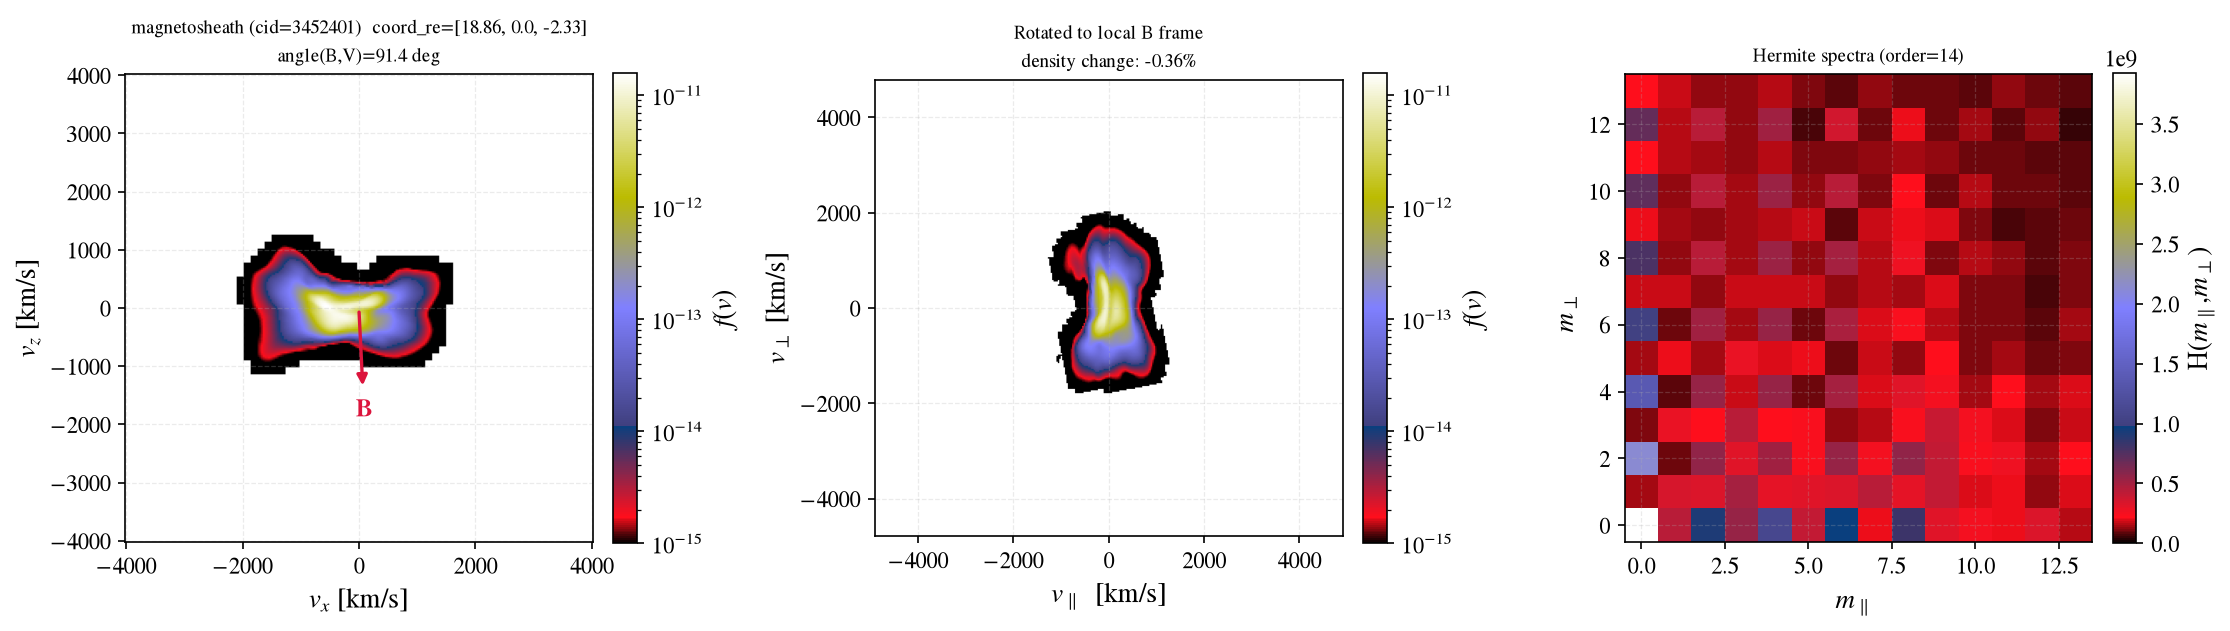
\includegraphics[width=\textwidth]{./images/vdf_rotation_hermite_magnetosheath.png}
\caption{Rotation and Hermite processing chain for the magnetosheath
representative (cid=3452401), smoke\_test run. Left: raw VDF
$v_x$--$v_z$ slice, with the in-plane direction of $\mathbf{B}$ (red
arrow) and the angle between $\mathbf{B}$ and the bulk flow annotated.
Center: the same VDF resampled into its local field-aligned frame
(Eq.~\ref{eq:rotation-frame}); the density change from interpolation
($-0.36\%$) is the rotation-correctness diagnostic. Right: its
log-space Hermite spectrum
(Eqs.~\ref{eq:hermite-projection}--\ref{eq:log-patch}), reduced to
$(m_{\parallel}, m_{\perp})$ by quadrature over the second
perpendicular index.}
\label{fig:rotation-hermite}
\end{figure}

Seven lower-order physical moments -- density,
3-component bulk velocity, 3-component anisotropic thermal velocity --
were computed in the same rotated frame and kept as separate features
(Section~\ref{sec:pca-prep}), since the Hermite transform's own
$u$/$v_{th}$ normalization deliberately strips out absolute
density/velocity/width.

% ---------------------------------------------------------------------
\section{PCA analysis}
\label{sec:pca}
% Blind PCA + KMeans clustering, scored against the physical labels
% from Section 1.

\subsection{Feature representation}
Results below use the \texttt{"hermite"} feature representation: each
sample's $14\times14\times14$ log-space Hermite spectrum
(Section~\ref{sec:data-processing}) flattened directly into a
2744-dimensional feature vector -- no slicing/downsampling, unlike the
\texttt{"raw"}/\texttt{"rotated"} pixel-slice representations, since the
Hermite basis already sees the full 3D VDF in a compact form.

\subsection{Feature preparation}
\label{sec:pca-prep}
Three preparation steps were applied, in this order, before
\texttt{StandardScaler}+PCA:
\begin{enumerate}
  \item \textbf{Per-sample normalization} (\texttt{sample\_normalization
    = "standard"}): each sample's flattened spectrum is mean-centered
    and divided by its own standard deviation. Physically structured
    populations (\texttt{current\_layer}, \texttt{magnetosheath}) have
    raw spectrum magnitudes $\sim$6--9$\times$ larger than quieter
    populations at the \emph{same shape} -- \texttt{StandardScaler}
    alone (per-feature column scaling) leaves each sample's own overall
    scale intact, so without this step that scale difference dominates
    variance ahead of any shape difference.
  \item \textbf{Moment features concatenated} (\texttt{include\_moment\_features
    = True}): the 7 moment columns from
    Section~\ref{sec:data-processing} are appended \emph{after} the
    per-sample normalization above, and are \emph{not} themselves
    per-sample-normalized -- they are exactly the absolute-scale
    information the Hermite transform's $u$/$v_{th}$ normalization
    discards, added back explicitly.
  \item \textbf{Post-\texttt{StandardScaler} moment weighting}
    (\texttt{moment\_feature\_weight = 10.0}): after
    \texttt{StandardScaler} gives every column unit variance, the 7
    moment columns are multiplied by $10\times$. Outnumbered
    $\sim$392:1 by Hermite columns (2744 vs. 7), their aggregate
    contribution to total variance would otherwise be diluted by column
    count alone, independent of how informative they are.
\end{enumerate}
PCA was fit with \texttt{n\_components = 40}; KMeans was fit for
$k \in \{2, \dots, 14\}$ and $k$ selected by silhouette score.

\subsection{Clustering results}
The silhouette score peaked at $k=2$ (0.314); scores for $k>2$ were
lower and comparable to each other (0.17--0.28, peaking again mildly at
$k=12$, 0.284) rather than showing a second clear elbow. Table
\ref{tab:cluster-composition} gives the $k=2$ cluster composition
against the ground-truth labels of Table \ref{tab:label-counts}.

\begin{table}[h]
\centering
\begin{tabular}{lrrrrrrr}
\toprule
Cluster & Size & lobes & magnetosheath & inner\_mag. & solar\_wind & current\_layer & undefined \\
\midrule
1 (disturbed) & 42 & 1 & 27 & 6 & 0 & 7 & 1 \\
0 (calm)      & 74 & 34 & 0 & 16 & 20 & 0 & 4 \\
\bottomrule
\end{tabular}
\caption{$k=2$ cluster composition, smoke\_test run, hermite features +
moments. Cluster 1 contains 100\% of \texttt{magnetosheath} (27/27) and
100\% of \texttt{current\_layer} (7/7) -- full recall of both
``disturbed'' substances -- at 81\% purity (34/42) within the cluster.
Cluster 0 is 100\% pure calm-plasma labels (\texttt{lobes}/
\texttt{solar\_wind}/\texttt{inner\_magnetosphere}/\texttt{undefined}),
zero contamination from either disturbed substance.}
\label{tab:cluster-composition}
\end{table}

Figures: \texttt{pca\_scatter.png} (first two PCs, colored by both
\texttt{cluster\_ml} and \texttt{cluster\_phys}),
\texttt{silhouette\_by\_k.png}, \texttt{cluster\_hermite\_spectra.png}
and \texttt{phys\_cluster\_hermite\_spectra.png} (flattened Hermite
spectra of representative samples, per PCA cluster and per physical
label respectively), all under
\texttt{data/plots/pca\_snapshot/smoke\_test/}.

\begin{figure}[h]
\centering
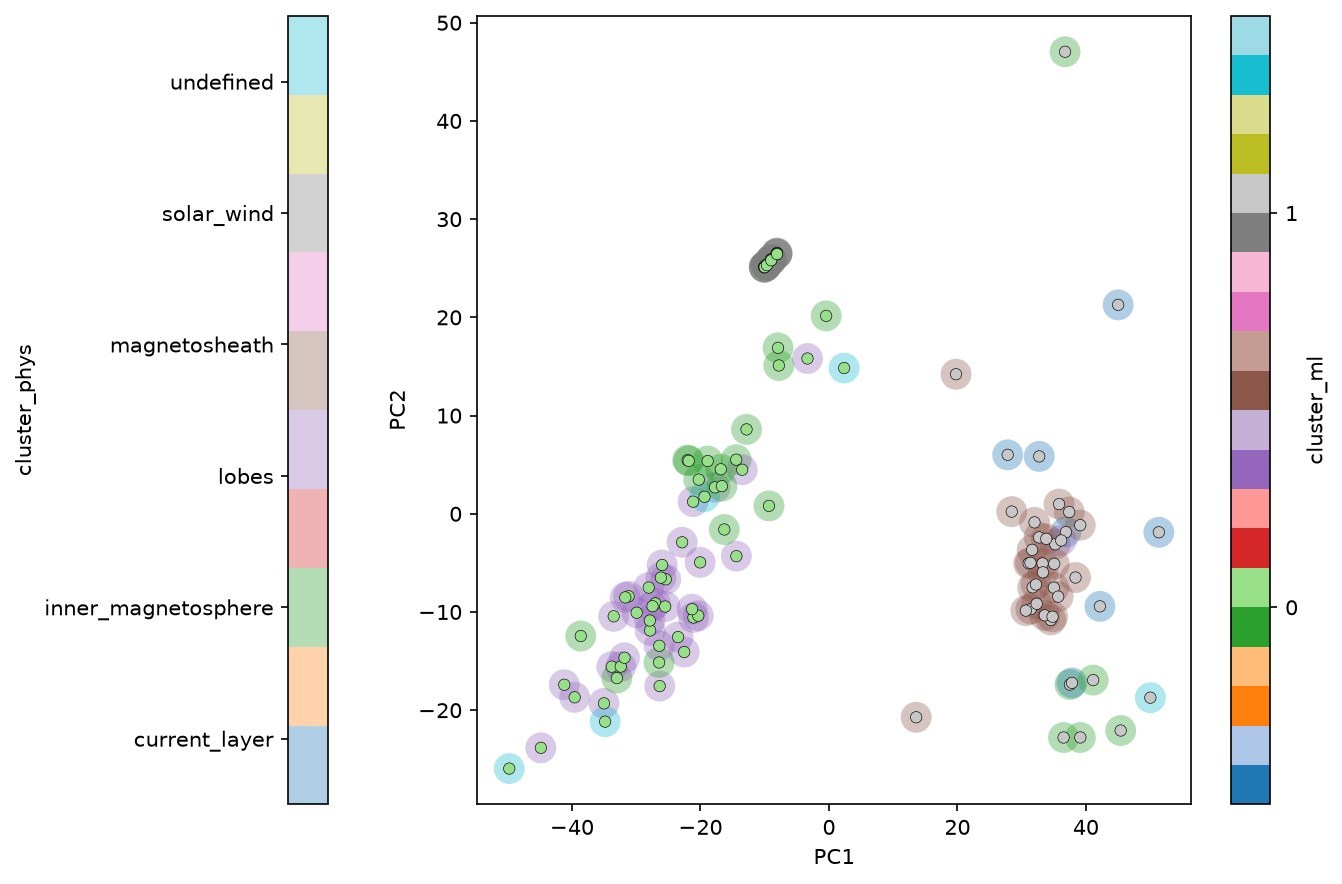
\includegraphics[width=0.85\textwidth]{./images/pca_scatter.png}
\caption{PCA scatter (first two principal components), smoke\_test run,
hermite features + moments, $k=2$.}
\label{fig:pca-scatter}
\end{figure}

\subsection{Discussion}
With this feature set, blind clustering reliably separates
``disturbed'' plasma (\texttt{current\_layer}, \texttt{magnetosheath} --
structured, non-Maxwellian VDFs) from ``calm'' plasma
(\texttt{lobes}/\texttt{solar\_wind}/\texttt{inner\_magnetosphere}/
\texttt{undefined} -- near-Maxwellian) with \emph{perfect recall} of
both disturbed substances at $k=2$: every \texttt{magnetosheath} and
every \texttt{current\_layer} sample lands in cluster~1, and cluster~0
has zero contamination from either. What it does \emph{not} yet do is
resolve substructure \emph{within} either tier -- silhouette scores for
$k>2$ don't show a clean second elbow, so KMeans on this feature set
doesn't naturally separate \texttt{magnetosheath} from
\texttt{current\_layer}, or \texttt{lobes}/\texttt{solar\_wind}/
\texttt{inner\_magnetosphere} from each other. The 19\% contamination in
cluster~1 (6 \texttt{inner\_magnetosphere} + 1 \texttt{lobes} + 1
\texttt{undefined}) is also worth a closer look at those specific
cells' spectra -- open question for the next iteration, not yet
investigated here.

% ---------------------------------------------------------------------
\section*{Appendix: run configuration}
\texttt{src/data\_proc/pipeline\_config.py}, as run for this report
(\texttt{RUN\_ID = "smoke\_test"}):
\begin{verbatim}
SPATIAL_BOXRE = [-30, 30, -5, 5]
POINTS_CONFIG["active_point_substances"] = ["current_layer"]
POINTS_CONFIG["current_layer_selection"]["core_fraction"] = 0.2
POINTS_CONFIG["current_layer_selection"]["min_r_re"] = 6.0
MAGNETOPAUSE_CONFIG["lobe_r_min_re"] = 10.0
BUILD_ROTATED_DATASET = False
BUILD_HERMITE_DATASET = True
HERMITE_ORDER = 14

PCA_CONFIG = {
    "n_components": 40,
    "k_range": list(range(2, 15)),
    "feature_representation": "hermite",
    "sample_normalization": "standard",
    "include_moment_features": True,
    "moment_feature_weight": 10.0,
}
\end{verbatim}

\end{document}
